\documentclass[paper=a4, fontsize=11pt]{article}
\usepackage{pdfpages}
\usepackage{parskip}
\usepackage{graphicx}
\usepackage[utf8]{inputenc}
\usepackage[english]{babel}
\usepackage[round,sort&compress]{natbib}
\usepackage{chemfig}
\bibliographystyle{unsrtnat}
\title{Plastics and the Environment}
\author{Joshua Reed}
\date{March 8, 2017}

\raggedright

\begin{document}
\maketitle
%Attach this form to the back of your issues research paper when you turn it in. Extras can be printed off the course webpage.


\section{Introduction}

Plastics are both vital to our economy and a major cause of concern regarding the health of humans, wildlife, and general pollution \cite{pl_en}.

Many plastics contain chemicals that are easily absorbed by human bodies. Some of these chemicals are known to effect human hormone levels.
Plastic is often found in aquatic life, and is therafter propagated throughout the food chain. 
Buried plastics can leach chemicals into ground water. A large portion of the worlds oil is used to create plastics. About 4\% of the worlds oil 
production becomes plastic, and nearly that much is used as energy in its production.

Still, plastic is a majore driver of economic action. Plastic production has ramped up massively over the years. Currently plastics are found in 
communications devices, cars, beverage containers, and yes the ubiquitous plastic bag. This begets a large part of the problem. Plastics are desired
for their excellent properties including durability; however, plastics are routinely used in disposable or even durable but short lived (compared to the lifespan
of plastics) products.

This paper's objective is to explore the issues created by plastics, and the economic benefits of using plastics. The history of plastics will be explored. 
A few case studies will be explored, and it will discuss the lifespan of plastics, 
the breakdown of plastics, alternative materials, and issues pertaining to the global adoption and use of plastics.

\section{Background}

\subsection{What is a plastic?}

According to Plastics Make it Possible, an American Chemistry Council funded website:

\textit{Plastics are simply chains of like molecules linked together. 
These chains are called polymers. This is why many plastics begin with “poly,” such as polyethylene, polystyrene, 
and polypropylene. Polymers often are made of carbon and hydrogen and sometimes oxygen, nitrogen, sulfur, 
chlorine, fluorine, phosphorous, or silicon.
The term “plastics” encompasses all these various polymers.
Although there are many polymers, plastics in general are lightweight with significant degrees of strength. 
Plastics can be molded, extruded, cast and blown into seemingly limitless  shapes and films or foams or even drawn into fibers for textiles. 
Many types of coatings, sealants and glues are actually plastics, too.}  \cite{what_plastics}

\subsection{History of Plastics?}

Bakelite was on of the first plastics similar to what we think of as plastics today.

\textit{ Bakelite, invented in 1907 by Leo H. Baekeland, an industrial chemist who had emigrated from Belgium. Celluloid came from a 
doughy mixture of nitrated cellulose (obtained from pulped paper or cotton) and camphor (from the bark of the Formosan camphor tree). 
Pressed into blocks under heat and pressure, it was sliced into thin sections and then, after being partially resoftened by heat, was cut, stamped, pressed, 
or molded into inexpensive consumer goods. Bakelite, the product of a condensation reaction between phenol and formaldehyde conducted under heat and pressure, 
was the first chemically synthetic plastic. When it first appeared as a substitute for shellac and hard rubber, it was used to mold electrical insulation.} \cite{hist_plastics}

Bakelite is still used in some forms today. Often the handle of a coffee carafe will be constructed of bakelite. 

Still a burgeoning industry, in 1925 Plastics recieved their first trade journal titled simply 'Plastics.' The signifigance of this is such that the term plastic wasn't widely
known or used.

In 1931 Plexiglas was invented. Plexiglas is a strong transparent type of plastic. Over the next two decades, various forms of plastics including Teflon, Nylon, ABS, Styrofoam, and even Kevlar.

While plastics have had many ups and downs, their use has become ubiquitous today.

In fact, according to the Center for Biological Diversity, In the first decade of this century, 
we made more plastic than all the plastic in history up to the year 2000. 
And every year, billions of pounds of plastic end up in the world’s oceans. \cite{biodiverse}

\subsubsection{Plastics in the Wild}

Plastics have been improperly disposed of for decades, and it's estimated that fish in the North Pacific injest 12-24,000 tons of plastic each year. \cite{biodiverse}
This plastic can harm
the fish internally, externally directly, and can cause issues with reproduction. 

These micro-plastics can work their way up the food chain. Sea turtles mistake plastic garbage for food, and have 
been found with soft plastic ropese, Styrofoam and monofilament lines in their stomachs.\cite{biodiverse}


To begin with, fish are a great resource for human consumption, but other impacts are less direct. A loss of biodiversity is bad for human's because it makes 
the world we live in less able to handle fluctuations in our ecosystems. \cite{biodiverse}

\subsubsection{Plastics and Human Health}
According to Envronmental Health News "Phthalates are used as plasticizers in the manufacture of vinyl 
flooring and wall coverings, food packaging and medical devices. Eight out of every ten babies, and nearly 
all adults, have measurable levels of phthalates in their bodies." \cite{ehn}

Plastics are classified as hazardous by the United Nations and have been shown to collect in the bloodstream. \cite{nature}

Still, plastics industry representatives insist that plastics are safe. Mike Neal, a consumer affairs representative at Plastics Europe 
has states "Every additive that we use is very carefully evaluated, not just by the industry, but also independently by government agencies to look at all the materials we use in plastics"

\subsubsection{Plastics and use of Fossil Fuels}
Of the oil produced globally, plastics use about 4\%, and yet another 4\% is used to process the plastic. \cite{eia}

As such, plastics use a large amount of our energy stores, and still cause pollution. One could argue however that plastics replace materials other materials that may take 
just as many resources. Either way, plastic consumption does contribute to \chemfig{CO_2} creation globally. 

As humans, the concenses is that \chemfig{CO_2} is one of the leading causes of global warming. 

\subsubsection{Plastics as a Disposable Product}
Products today aren't meant to last forever, or even many lifespans. This is a growing concern as the breakdown times of plastics is nowhere near the
product's lifespan. Plastic bags break down after 10-20 years, plastic bottles about 100, monofilament fishing lines over 
600.\cite{super}

Still, we use plastics in products with short life spans such as computers and cell phones, but even in products with ultra-short lifespans such as the plastic fork.

The really scary part is that once plastics are in the wild, there's no filtering them back out.

Again, industry representatives claim these plastics are safe, and to be fair there have been efforts to recycle plastic products.

\section{View points}

\subsection{Use Plastics as an Economic Driver}
Plastics are an economic driver and can be used responsibly. Using plastic instead of glass can actually save energy by up to 
55\%. \cite{ehn}

Solar water heaters using plastics can also provide up to two-thirds of a households kannual hot 
water. \cite{what_plastics}

\subsection{Regulate Plastics as a Pollutant}
One viewpoint is that plastics should be classified as hazardous waste. 

Plastics that do break down into smaller and smaller pieces are digested by wildlife.

This way it enters food webs and due to magnification, it can actually be in higher concentration at the 
tops of the food chains more so than the bottoms. 
These plastics can harm reproductive systems.

Beyond the digestion of plastics, plastics themselves when disposed of the same way as food scraps--the way they are treated in 
the United States, Europe, Australia, and Japan can either leach chemicals into ground water, or worse make their way into other
habitats. 

As can be seen in the two images below, plastics can also physically harm an animal or habitat. 

\begin{figure}[ht!]
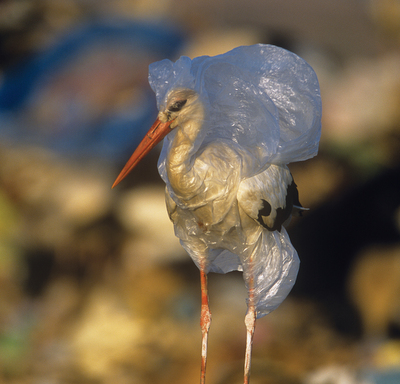
\includegraphics[scale=.5]{plastic_bird.jpg}
\caption{Bird Trapped in Plastic Bag \cite{long_term}}
\end{figure}
\cite{long_term}

\begin{figure}[ht!]
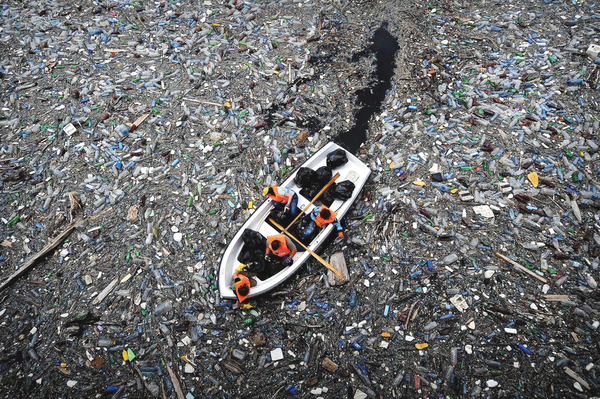
\includegraphics[scale=.5]{plastic_river.jpg}
\caption{Navigating a River of Plastic \cite{long_term}}
\end{figure}



\section{Conclusion}

\subsection{Recap of the Issues}

Plastics are excellent materials. They are almost magic. Unfortunately the way plastics are treated in our modern times leads to high
levels of pollutants. 

Beyond that, plastics can pose a risk to human health, and often times plastics contain additives that haven't been throroughly tested--as was the case 
with BPA. Plastic pollutants can also make their way into wildlife and cause great damage there. Still plastics have decent uses, and can even be a part
of the solution regarding environmental concerns.

\subsection{Solutions}
Regulations can make plastics recycleable by nature, people can take action to recycle plastics used, and products containing plastics can laber their products bio-degradation
times. Plastics aren't going away, and there are efforts to create biodegradable plastics through so called 'green chemistry.'
There are solutions! 


\bibliography{Plastics}


\end{document}  
